\section{The \SYSTEM{} Protocol} \label{sec:approach}

In this section, we describe the components of the \SYSTEM{} protocol, step
through each in detail, and then introduce our proof-of-concept implementations
of these components.

\subsection{Participants}

\noindent\textbf{Provider.} The \emph{provider} is the entity in control of both
the server and backend with the goal of ensuring the integrity of resources
downloaded from their system. \\

\noindent\textbf{\SYSTEM{} Frontend.} The \emph{frontend} is responsible for
calculating the Uniform Resource Name (URN) and Backend Domain (BD) of the
resource downloaded from the server. Afterwards, the frontend queries the
backend using this URN and, if an integrity violation is detected, quarantines
the resource and warns the user. \\

\noindent\textbf{Server.} The \emph{server} is a distribution system (hopefully)
controlled by the provider that hosts resources for download. It can be internal
or external, a single server or many, first-party or third-party. \\

\noindent\textbf{\SYSTEM{} Backend.} The \emph{backend} is responsible for
advertising a queryable listing of URNs that \SYSTEM{} frontends can use to
judge the legitimacy of downloads. It is a high availability system that is
wholly separate from the server (not co-hosted) and controlled by the provider.

\subsection{Protocol Overview}

\begin{figure}[ht]
    \centering
    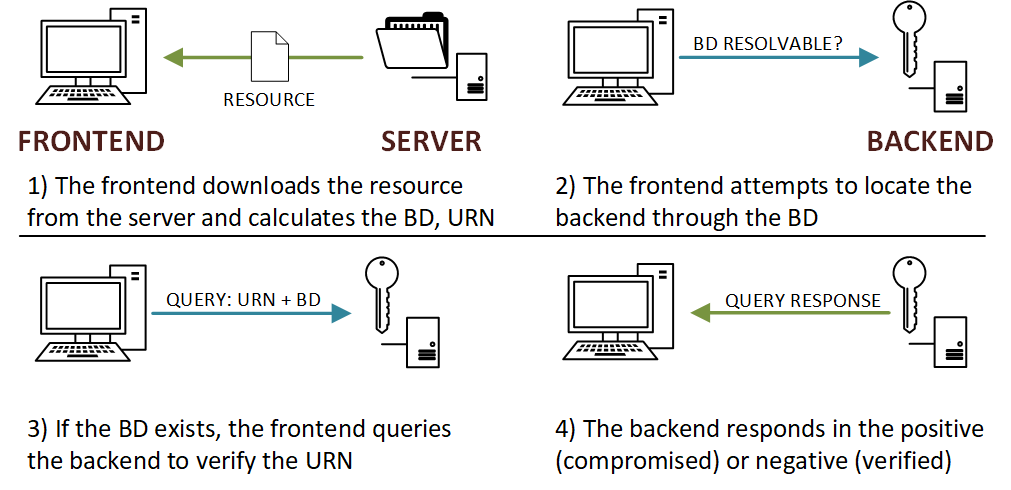
\includegraphics[width=\linewidth]{haschk-overview.png}
    \caption{A high level overview of the (generic) automated checksum
    verification process beginning when a user downloads a
    resource.}\label{fig:protocol}
\end{figure}

\figref{protocol} gives a high level overview of the \SYSTEM{} protocol.
Initially, when a user finishes downloading a resource from the provider's
server, the frontend runs the resource's contents through a SHA-256 hashing
function, yielding a 256-bit digest. Any hashing function can be used so long as
it is pre-image and collision resistant~\cite{Rogaway}. This digest is used to
construct a hash-based Uniform Resource Name (URN) uniquely identifying the
resource. Additionally, a Backend Domain (BD) is derived from the domain name of
the server. The frontend uses the BD in an implementation-dependent manner to
locate and query the backend, checking for the existence of the constructed URN
and essentially asking: \emph{``is this a compromised resource?''} If the URN is
found, a negative response is returned indicating a verified resource. If the
URN is not found, a positive response is returned indicating a compromised
resource.

If the query returns a positive response: (1) the user should be warned pursuant
to the recommendations of Akhawe et al~\cite{Akhawe} (avoid warning fatigue, be
invisible), Cherubini et al~\cite{Cherubini} (simple non-technical language,
secure default action), Modic et al~\cite{Modic} (issue warnings from a position
of authority), and others; (2) the download should be deleted, renamed, or
otherwise made inaccessible/quarantined by default; and (3) the user should
still be allowed to ``click through'' and override the warning and the default
quarantine behavior, though ideally this should be less convenient than the
default action~\cite{Cherubini}.

If the query returns a negative response, the frontend should indicate this
inconspicuously to mitigate the threat of warning/popup
fatigue~\cite{Akhawe, Cherubini} and habituation~\cite{Sunshine}. For example,
our frontend implementation simply changes its icon when downloads are
successfully verified and only issues popup warnings when compromised downloads
are positively identified.

To prevent false positives, integrity checking is skipped if the backend's
location is unresolvable or \SYSTEM{} is not properly deployed. Determining when
this is the case is implementation-dependent. To prevent false-negatives, when
\SYSTEM{} is properly deployed and a URN is not found during lookup, the backend
response will always be interpreted as positive. As a result, it is not possible
to only secure ``some'' resources on a server.

\subsubsection{Deriving the Backend Domain (BD)}

Before we can communicate with a provider's backend, we require some scheme to
locate it. We refer to this scheme as deriving the \emph{Backend Domain} (BD).
The BD is some identifier that allows the frontend to locate the backend. For
our Domain Name System (DNS) based implementation (below), the BD is the
Third-Level Subdomain (3LD) or Second-Level Domain (2LD) based on the server
URI's host subcomponent~\cite{RFC3986} and are queried in that order. \\

Example 1: an FTP frontend (\eg{ Filezilla, Transmit, et cetera}) downloading a
resource from an FTP server at
\texttt{ftps://un:pw@ftp.example1.com:8080/some/resource} has a host
subcomponent of \texttt{ftp.example1.com} and a BD of \texttt{ftp.example1.com}
or \texttt{example1.com}. \\

Example 2: a browser frontend (\eg{ Lynx, Google Chrome, Internet Explorer, et
cetera}) downloading a resource at \texttt{https://s4.l.cdn.example2.com/fl}
from a hyperlink on the page \texttt{https://dl.app.example3.com/index/page} has
a host subcomponent of \texttt{dl.app.example3.com} (\emph{not
\texttt{s4.ll.cdn.example2.com}}) and a BD of \texttt{app.example3.com} or
\texttt{example3.com}. \\

It is important that the right BD is derived to ensure correct operation of the
protocol. This concern is implementation-dependent. Specifically, in the case of
the browser frontend in example 2 (above), the BD is not derived from the
resource's URI directly but from the URI of the HTML page containing the
hyperlink pointing to that resource. This prevents an adversary from trivially
fooling \SYSTEM{} by, for instance, replacing
\texttt{https://s4.l.cdn.example2.com} with a hyperlink pointing to
\texttt{https://attacker.com} and hosting a conforming \SYSTEM{} backend that
would cause the frontend to respond with a false negative.

Further, depending on the implementation, a frontend or backend may not be using
URIs and DNS to transact information over the internet at all. An example of
this is a purely Distributed Hash Table (DHT) based backend. In such a case, any
derivation algorithm (or no derivation at all, \eg{ the BD is hardcoded}) can be
used as long as correct operation of the protocol is ensured.

\subsubsection{Constructing Uniform Resource Names (URN)}

To ensure the integrity of arbitrary resources, we require some method to
uniquely and durably identify those resources. We accomplish this through the
adoption of the informal IETF draft for the construction of hash-based
\emph{Uniform Resource Name} (URN) namespace~\cite{draft-URN}, which the
frontend follows when calculating URNs for each resource downloaded. Through
whatever implementation-specific method, the backend must ``advertise'' or allow
lookups against a set of expected URNs corresponding to the resources hosted on
the provider's server, even if those resources have unstable access paths or
URIs; \eg{, when resources are hosted externally, on download mirrors, on CDNs,
et cetera}. This requirement is satisfied by implementations combining URNs with
the BD, thus durably associating the URNs calculated in the frontend with the
URNs advertised by a provider's backend regardless of where the corresponding
resources are hosted on the provider's server.

Since the backend advertising URNs is \emph{never} co-hosted alongside the
system that distributes the corresponding resources---like a web or FTP
server---\SYSTEM{} retains the ability to protect users from dangerous downloads
\emph{even when the system distributing the resource has been completely
compromised}. This is not true of prior approaches to automated checksum
verification of arbitrary resources~\cite{Cherubini}.

\subsection{Protocol Implementation}

We implement a proof-of-concept \SYSTEM{} frontend as a Google Chrome extension.
To demonstrate the general applicability of our approach, our frontend currently
works with two backends: (1) directly with DNS via Google's JSON API for DNS
over HTTPS (DoH) and (2) indirectly with DHT (Ring OpenDHT) via a local
Representational State Transfer (REST) API we designed to mimic the response
syntax of Google's DoH JSON API. Other candidate backends include storage
clusters, relational and non-relational databases, and any high availability
key-value store.

Our extension operates following the high level overview in \figref{overview}
with some key implementation-specific functionality that we explore in the
remainder of this subsection. After the user initiates a download either
directly (\eg{ typing a URI manually}) or by following a hyperlink, our
extension, having observed the initial web request, associates that request with
the new download item. The original request may have directly triggered the
download or the download may have been triggered after one or more redirections.
Our extension derives the correct BD in both cases (see below). At this point,
if the backend does not exist or does not conform to the protocol, the protocol
terminates. Otherwise, after the download completes, a URN is calculated and
combined with the BD to make a final query to the backend. In effect, this query
asks: \emph{is this resource compromised?} If the response to the query is
negative (\ie{ a DNS TXT record or DHT data value}), the extension considers the
resource validated. On the other hand, if the response to the query is positive
(\ie{ no record found or bad data value returned}), the extension considers the
resource compromised, deletes the resource file, and warns the user.

In keeping with UX suggestions of prior work, our extension is virtually
transparent to end users in the common case that a download is successfully
verified by a provider's backend or when \SYSTEM{} has not been properly
deployed by a provider. However, in the relatively uncommon case that a resource
is deemed compromised, the extension will delete the file and alert the user
with the primary option to ``dismiss'' the alert, mimicking Chrome's own highly
effective dangerous download warning~\cite{ChromeClickThrough}. Specifically:
the user has the option of clicking through the warning via a low-key secondary
interface where they can force the extension to ignore the compromised nature of
the resource \emph{the next time it is downloaded}, forcing the user to trigger
the download again. This inconvenience, favoring users' security over choice, is
in keeping with the recommendations of prior work regarding security warning UX
(see \secref{introduction}).

As no JavaScript OpenDHT client implementation exists, we developed a REST API
to facilitate communication between our extension and the Ring OpenDHT network
via HTTP and JSON. In a production implementation, a JavaScript OpenDHT client
would be baked directly into the extension.

Deploying the DNS backend is as simple as adding certain TXT records to our DNS
zone. This is a straightforward operation. Similarly, deploying the DHT backend
requires adding certain key-value to the OpenDHT network, which is trivial.
Moreover, both DNS and DHT backends are performant and highly available. The
Ring OpenDHT network is also free to use. In the case of DNS, the vast majority
of web-facing providers and IT teams are already using it, already pay for their
own DNS zones, and are already quite familiar with configuring and managing
them. Hence, no exotic secondary backend system is required for providers with
web servers. Additionally, we argue updating the URNs stored by these backends
automatically---by integrating a URN calculation and record insertion/update
step into a modern development toolchain or resource deployment pipeline---is
relatively low-effort and straightforward for providers.

No application or website source code changes, costly user-facing server or web
infrastructure customizations, or modifications to web standards are needed to
enable our extension to protect a provider's resources. Given a production-ready
implementation of our frontend---coupled with the near ubiquitous adoption of
DNS---\SYSTEM{} (with a DNS backend) could be deployed immediately by interested
providers.

\subsubsection{URNs, BDs, and Fallthrough in Google Chrome}

BD derivation in the browser is non-trivial. Users can initiate downloads
through clicking links inside \emph{and outside} the browser (\eg{ in an email
application}), through asynchronous JavaScript, and by entering URIs into the
browser manually. To catch these and other edge cases, we implement our
extension using the WebRequest API~\cite{ExtensionAPI}, which allows us to
monitor all navigation events, collate redirects into an interrogable chain of
requests, and associate new download items with the URI where they were
originally initiated.

To query the backend, we: (1) BASE32 encode the resource's URN. (2) Divide the
112-character result into two 56-character strings \texttt{C1} and \texttt{C2}.
(3) We calculate the BD, which is either the 3LD and 2LD from
\texttt{details.originUrl}. We choose by issuing up to two queries of the form
\texttt{AL.BD}, where the Application Label (AL) is the constant string
\texttt{\_haschk}, looking for a response containing the value \texttt{OK}. We
first query the 3LD as BD and, if we do not receive the proper response there,
query the 2LD as BD. If the proper response is not received from either query,
the extension assumes \SYSTEM{} has not been properly deployed and terminates.
(4) Otherwise, concatenating C1, C2, AL, and BD, we issue a query of the form
\texttt{C1.C2.AL.BD}, again looking for a response containing \texttt{OK}
(negative) or that the query was not found (positive).

To handle redirection, we use Chrome's Web Request API to associate redirected
requests with one another. The originating request's \texttt{origin} at the top
of this chain is used to derive the BD using the \texttt{details.originUrl} and
\texttt{details.documentUrl} properties (also avoiding iframe issues). This
prevents an adversary from trivially fooling \SYSTEM{} by replacing a legitimate
hyperlink with a malicious one. A naive implementation might use the
\texttt{DownloadItem.referrer} property to derive the BD, since it should be
populated with the originating URL. Unfortunately, this property can be
manipulated with one or more redirections causing the BD to point into the
attacker's DNS zone. If the attacker properly deploys a \SYSTEM{} backend, they
could then trivially force false negatives.

Keeping a chain of associated requests also allows us to implement
``fallthrough'' functionality where, if the original request at the head of the
chain has not deployed \SYSTEM{}, the extension can walk the chain, checking
each point of redirection for a proper \SYSTEM{} deployment. This would ensure
URL shorteners and other redirection services do not trigger false positives.
